\documentclass{amsart}
\usepackage[margin=3cm]{geometry}                % See geometry.pdf to learn the layout options. There are lots.
\geometry{letterpaper}                   % ... or a4paper or a5paper or ...
%\geometry{landscape}                % Activate for for rotated page geometry
\usepackage[parfill]{parskip}    % Activate to begin paragraphs with an empty line rather than an indent
\usepackage{float}
\usepackage{graphicx}
\usepackage{amssymb}
\usepackage{epstopdf}
\usepackage{siunitx}
\usepackage{subcaption}

\DeclareGraphicsRule{.tif}{png}{.png}{`convert #1 `dirname #1`/`basename #1 .tif`.png}

\title{      }
\author{Caspar \textsc{Lant}} % Author name

\date{\today} % Date for the report

\begin{document}

\bigskip

\maketitle % Insert the title, author and date
\begin{center}

Intermediate Experimental Physics II\\
\vspace{1.5cm}

\begin{tabular}{l r}

Section: & 002\\
\\
Date Performed: & February 2, 2015 \\ % Date the experiment was performed
Date Due: & Februrary 9, 2015\\
\\
Partner: & Sam P. Meier \\ % Partner names
Professor: & Prof. Andrew Kent\\
Instructor: & David Mykytyn % Instructor/supervisor
\end{tabular}
\end{center}
\vspace{50mm}
\pagebreak

\paragraph{\textbf{The Objective} of this week's experiment was to put our vast theoretical knowledge of lenses to application. It is always a remarkable think to see what was once pure abstraction validated though rigorous scientific experimentation. }

\section{Theoretical Background/ Abstract}
\paragraph{Just over a century ago, Danish physicsist and renowned goalkeeper Niels Bohr postulated the discrete nature of the energy states available to the sole electron in the hydrogen atom. }
\begin{equation}
\frac{1}{s_i}+ \frac{1}{s_o} = \frac{1}{f}
\end{equation}
\begin{equation}
\frac{1}{f} = (n-1)\Big(\frac{1}{R_1} - \frac{1}{R_2}\Big)
\end{equation}

\section{Experimental Procedure}
\begin{enumerate}
\item Carefully remove the extremely expensive tube from its bubble wrap cocoon.
\item Delicately slot the tube into the socket of the supplied cable, and place it in the oven.
\item Attach the other end of the cable to the propriety apparatus
\item Do not break the tube! It's expensive!
\item Turn on the measurement apparatus, as well as the oscilloscope.
\item Set the switch to reset.
\item Set the value of $U_3$ to 1.5V.
\item Wait about 20 minutes for the Frank-Hertz tube to reach its operating temperature $\vartheta_s = 188^{\circ}$.
\item Turn the largest dial to the sawtooth position, and dial $U_1$ and $U_3$ such that the function displayed on the 'scope approximates the curve found on the last page of the instruction packet.
\item Set up DataStudio with voltage sensors A and B connected to the oscilloscope inputs.
\item Create a graph of voltage B vs. voltage A.
\item Send a single sawtooth wave into the DataStudio interface by using the dial on the Frank-Hertz power supply. You should see a more detailed view of the initial oscilloscope trace on your DataStudio display.
\item Calculate the distance between two peaks using DataStudio's wonderfully intuitive interface! This should come to about 4.9V; the value postulated by Niels Bohr well before your grandparents were alive.
\item You're done! Don't break the tube!
\end{enumerate}

\section{Graphs and Calculations}

\begin{figure}[H]
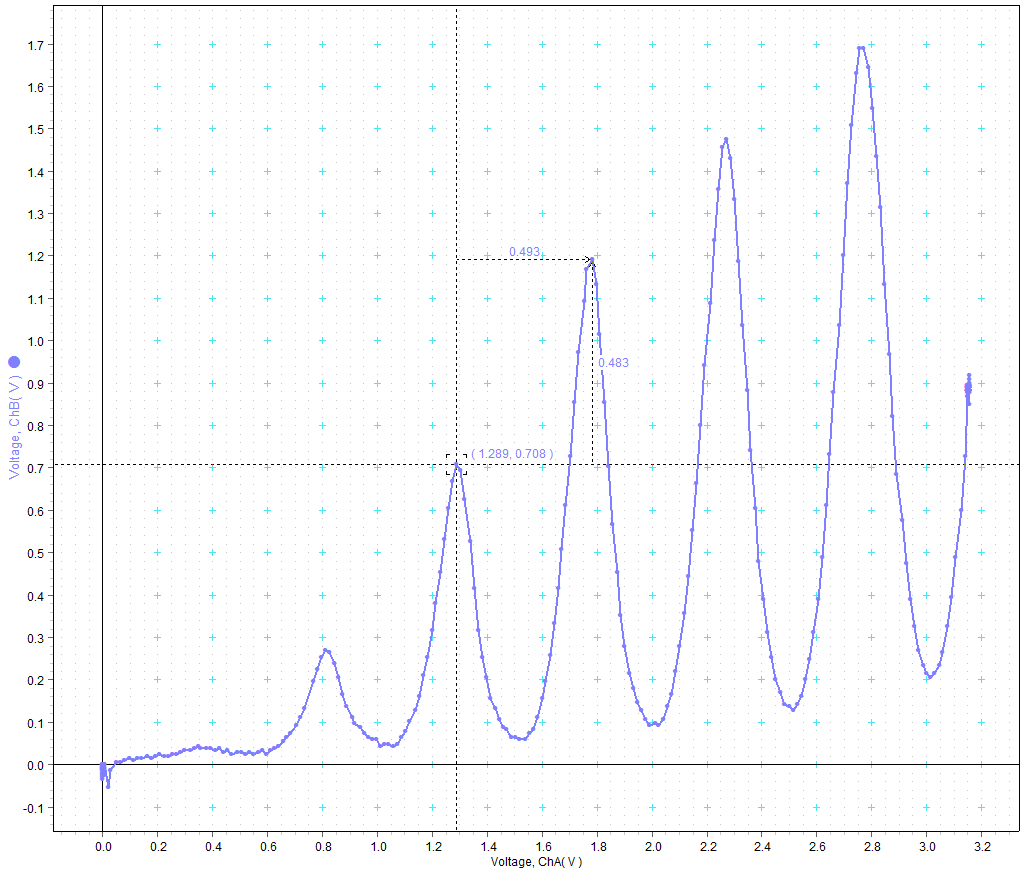
\includegraphics[width=0.9\textwidth]{graph.png}
\caption{Discrete Energy Levels at Intervals of 4.9V}
\end{figure}

\begin{figure}[H]
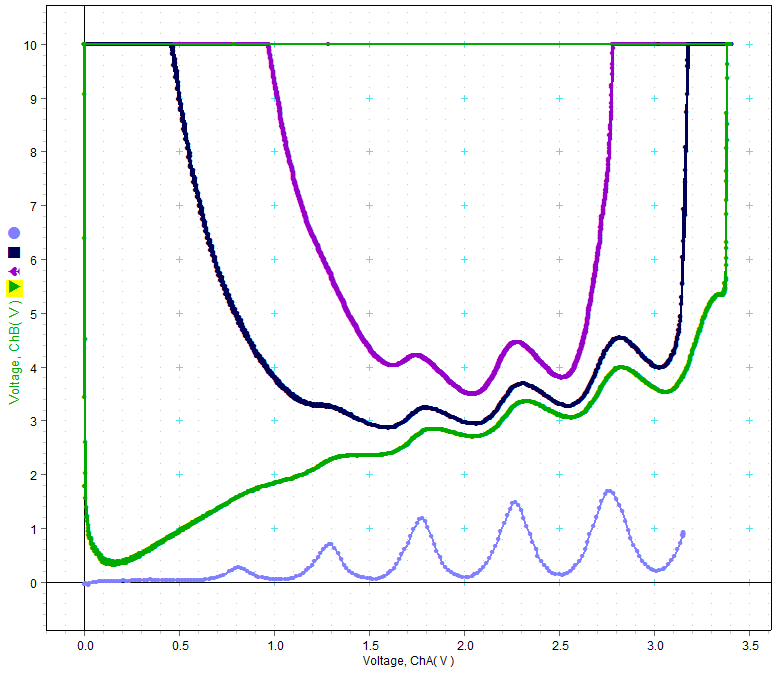
\includegraphics[width=0.9\textwidth]{saturation.png}
\caption{Saturation}
\end{figure}

\medskip

\pagebreak


\section{Graphs and Calculations}

\begin{figure}[H]
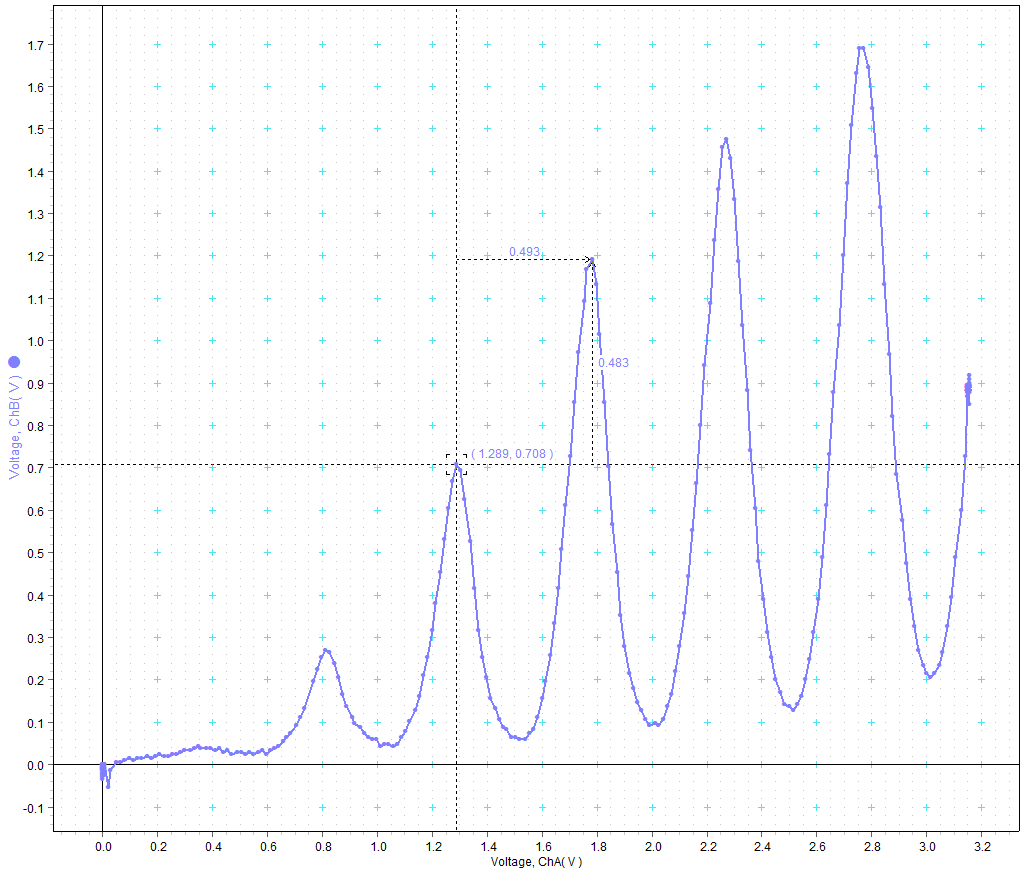
\includegraphics[height=0.42790985\textheight]{graph.png}
\caption{Discrete Energy Levels at Intervals of 4.9V}
\end{figure}

\begin{figure}[H]
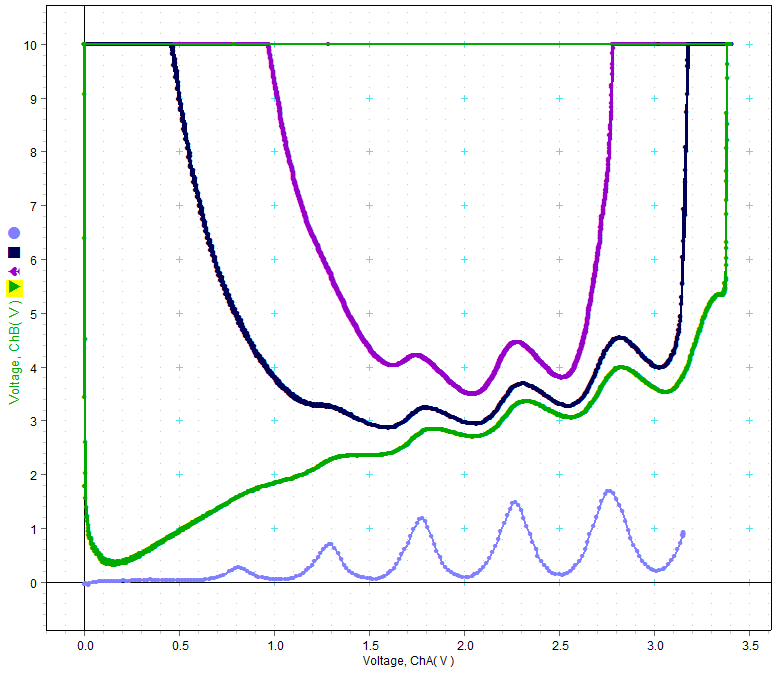
\includegraphics[height=0.42790985\textheight]{saturation.png}
\caption{Saturation}
\end{figure}

\medskip

\pagebreak

\section{Questions}

\begin{enumerate}
\item {\textit{Why is it better to have the cathode indirectly heated rather than directly heated?}
\begin{quote}
It is easier to regulate the temperature of the hot cathode if it is heated indirectly. The junction between the heater and the cathode acts as a buffer against fluctuating currents.
\end{quote}}

\item{\textit{When the oven temperature is too low, why is there the possibility of a discharge?}
\begin{quote}
The logarithm of the vapor pressure of a substance is inversely proportional to its temperature. It is important that we run our experiment at sufficiently high temperatures, and low enough corresponding vapor pressure such that vaporized mercury atoms are well-dispersed throughout the tube.
\end{quote}}

\item{\textit{Why should the oven temperature not be too high?}
\begin{quote}
If the oven temperature is too high, we run the risk of damaging the extremely expensive tube at enormous cost. Neglecting glass-breakage, too high a temperature would result in a reduction of the mean-free path of our electrons. This means, physically, that our electrons would experience too many collisions for the experiment to produce any observable effects of quantum energy states.
\end{quote}}

\item{\textit{Does the first peak occur at (U1 + U2) = 4.9 V? Can you think of reasons as to why it would not?}
\begin{quote}
I'd say that this engima was due to the presence of the ocilloscope in our circuit. The device drops a constant voltage between the output of the power supply and our lab interface. This has the effect of lowering the voltage at which the first spike occurs, and has no bearing on the distance between consectutive spikes, invariably 4.9V.
Revision: I went back into the lab and ran the experiment again, this time with the oscilloscpoe off. The presence of the oscilloscope in my circuit seems only to affect the voltage of the peaks, and not the voltage at which the peaks occur. See the digram below: The data in brown was collected with the oscillospe on, and the data in blue was not.

\begin{figure}[H]
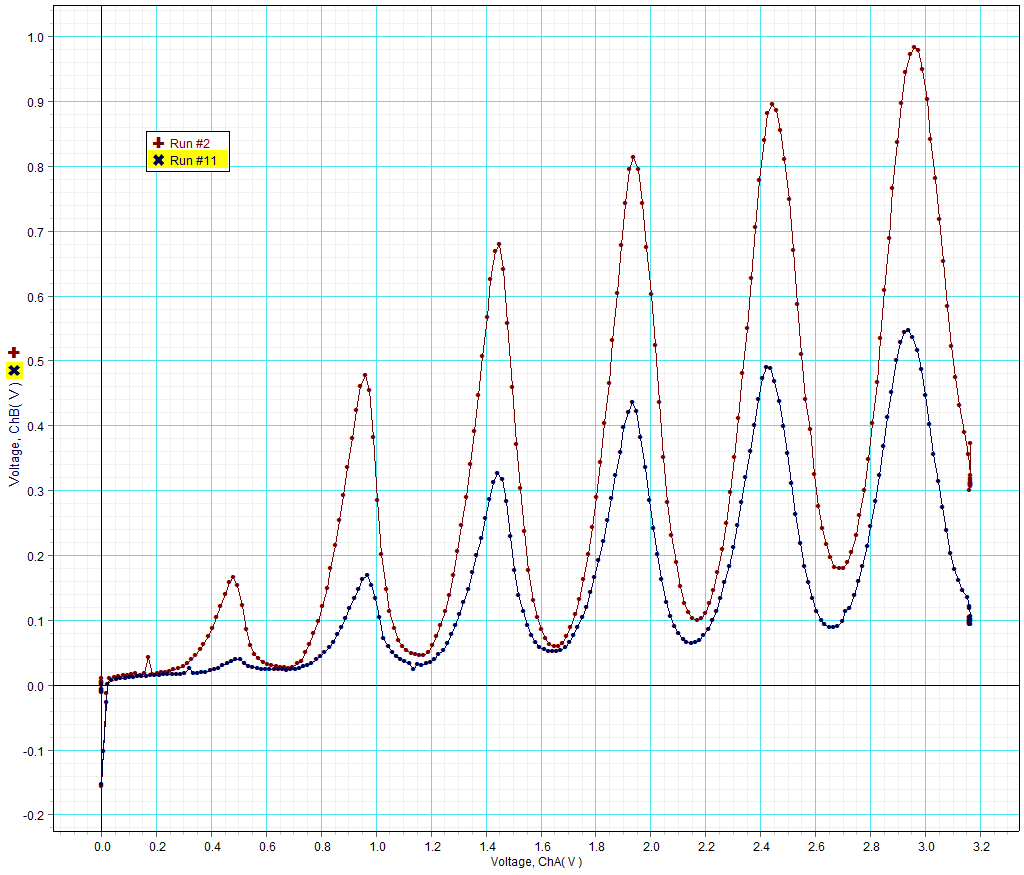
\includegraphics[height=0.42790985\textheight]{scopeoff.png}
\caption{NoScope!}
\end{figure}

You'll This was again confirmed when I probed the oscilloscope terminals with a multimeter with the Frank-Hertz powered down, and found a voltage drop of effectively zero, as shown in the photo below
\end{quote}}
\end{enumerate}

\section{Error Analysis}




\end{document}
t
